\subsection{Concept drift}

The problem of \textbf{concept drift}\sidenote{Concept drift} describes how a process changes over time. A good example is ice cream sales throughout one year. As one can see in \ref{fig:7_cd_ice_cream}: Within one year the curve heavily peaks over the summer months, but the curve is stable over the years.

\begin{figure}[H]
  \centering
  \begin{subfigure}{0.5\textwidth}
    \centering
    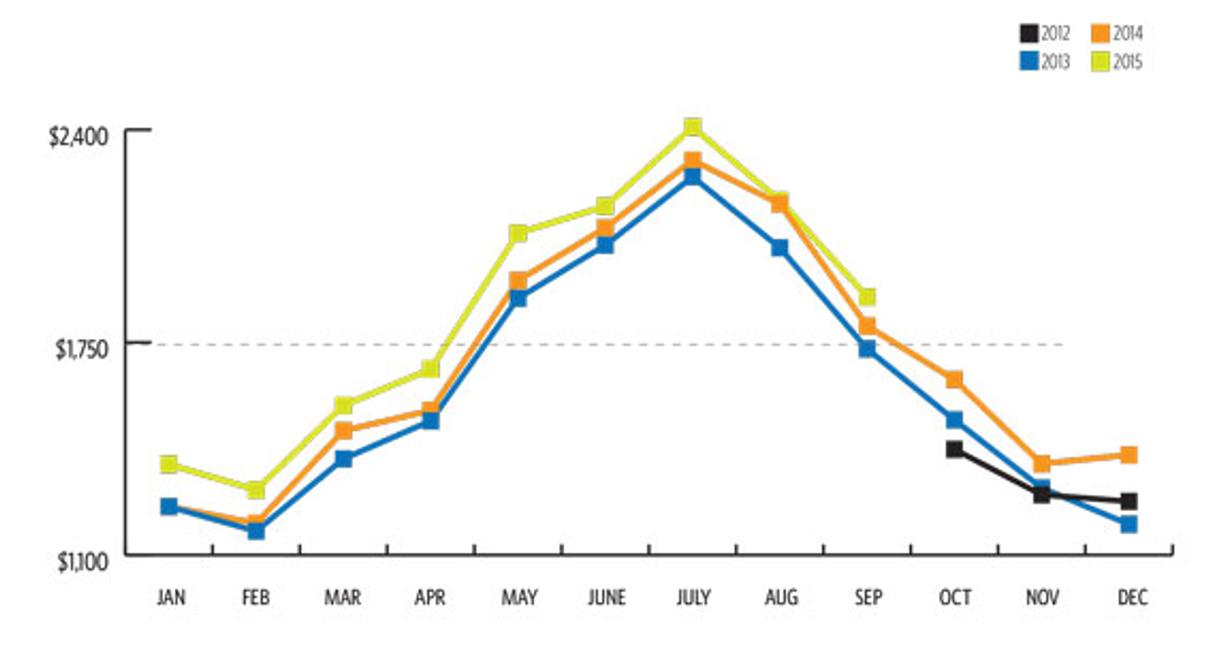
\includegraphics[width=\textwidth]{assets/sl/cd__ice_cream.png}
  \end{subfigure}

  \caption{Process changing over time: example ice cream sales}
  \label{fig:7_cd_ice_cream}
\end{figure}

Whenever trying to describe a model, the following questions are important:
\begin{itemize}
  \item What should the model describe? Which time frame? \begin{note}(E.g. last year, last decade, ...)\end{note}
  \item When predicting, is it better to use only recent data or also include older data? (drift $\leftrightarrow$ sparsity)
\end{itemize}

\begin{figure}[H]
  \centering
  \begin{subfigure}{0.4\textwidth}
    \centering
    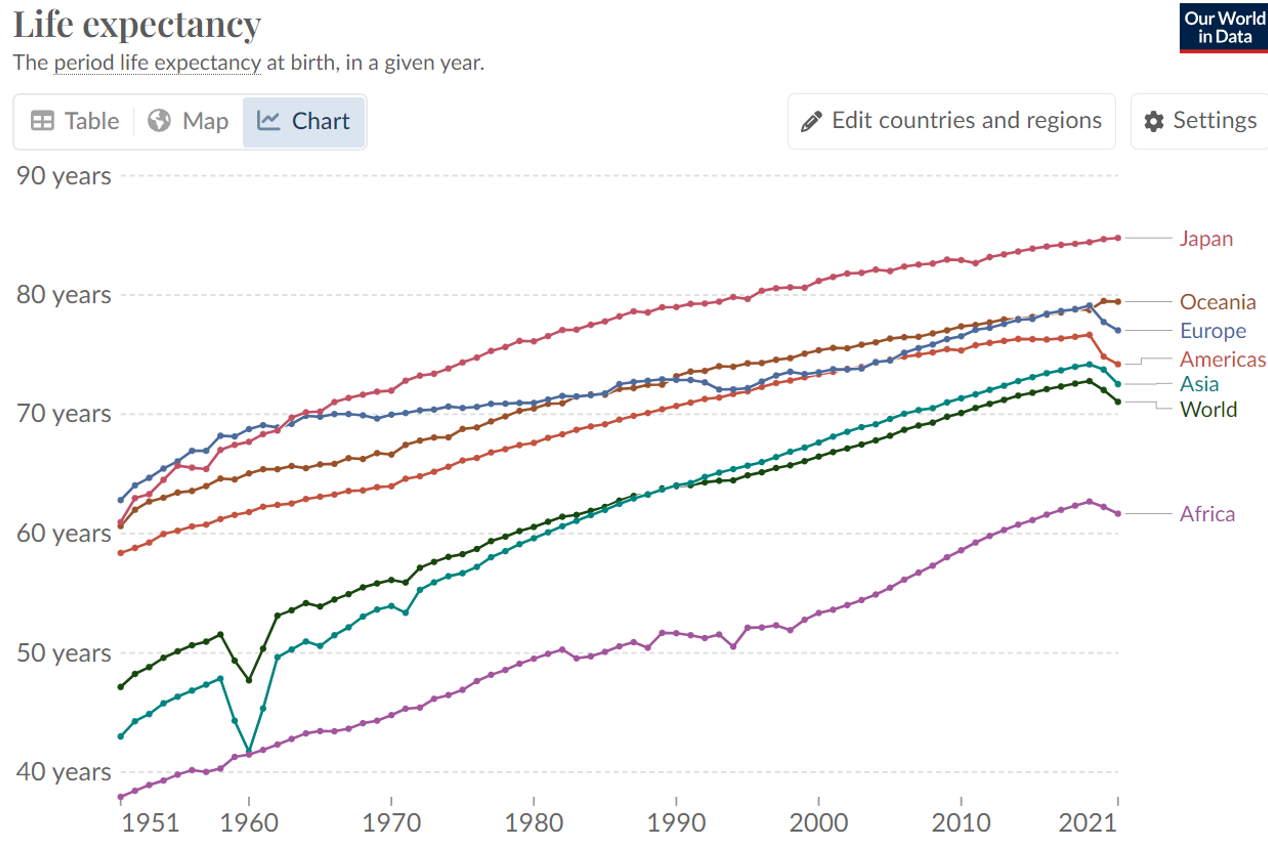
\includegraphics[height=3.5cm]{assets/sl/cd__example_1.png}
  \end{subfigure}
  \hspace*{0.05\textwidth}
  \begin{subfigure}{0.4\textwidth}
    \centering
    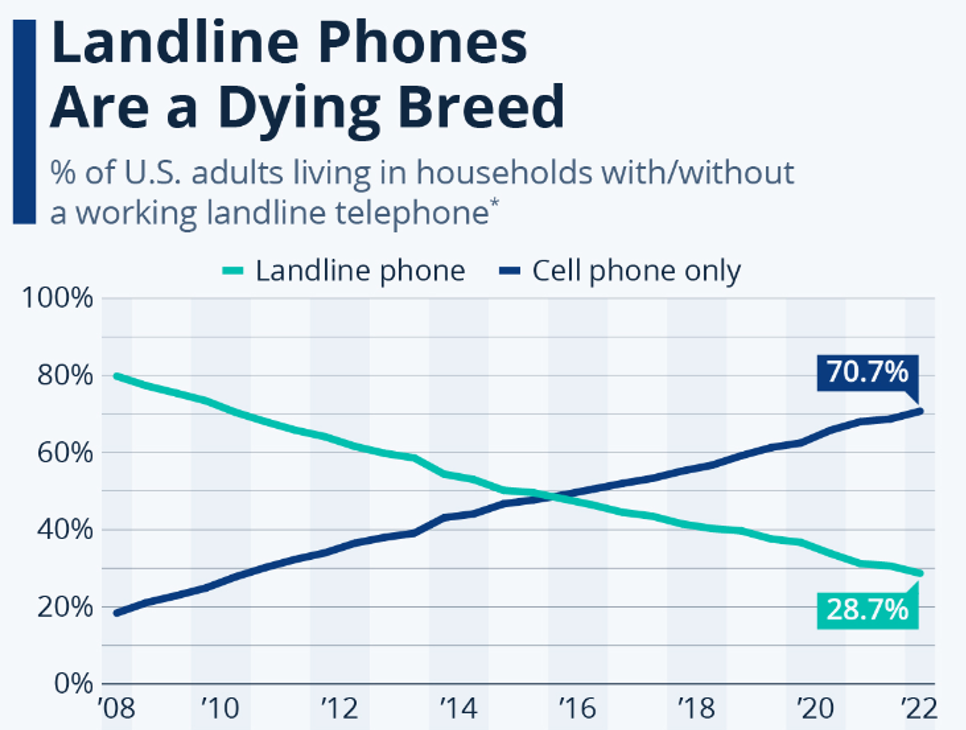
\includegraphics[height=3.5cm]{assets/sl/cd__example_2.png}
  \end{subfigure}

  \caption{Concept drift: time dependency examples}
  \label{fig:7_cd_include_before}
\end{figure}

To have a measure of how much drift is even involved in given data, we use the \textbf{system stability index (SSI)}.
\begin{align*}
  SSI\sidenote{System Stability Index} = \sum_{c \in classes}\Big(
    \underbrace{\frac{|\mathcal{A}_{t=c}|}{|\mathcal{A}|}}_{\begin{array}{c}
      \scriptstyle\text{fraction of instances}\\
      \scriptstyle\text{in \textbf{original test set}}\\
      \scriptstyle\text{classified as }c
    \end{array}} -
    \underbrace{\frac{|\mathcal{B}_{t=c}|}{|\mathcal{B}|}}_{\begin{array}{c}
      \scriptstyle\text{fraction of instances}\\
      \scriptstyle\text{in \textbf{new data set}}\\
      \scriptstyle\text{classified as }c
    \end{array}} 
  \Big) \cdot \log_e
  \Big(
    \frac{|\mathcal{A}_{t=c}|}{|\mathcal{A}|} /
    \frac{|\mathcal{B}_{t=c}|}{|\mathcal{B}|}
  \Big)
\end{align*}
\begin{itemize}
  \item Informal interpretation: $\begin{array}{rl}
    SSI < 0.1 & \text{no significant drift}\\
    0.1 \leq SSI < 0.25 & \text{moderate drift}\\
    0.25 \leq SSI & \text{significant drift}
  \end{array}$
\end{itemize}

\begin{figure}[H]
  \centering
  \begin{subfigure}{0.8\textwidth}
    \centering
    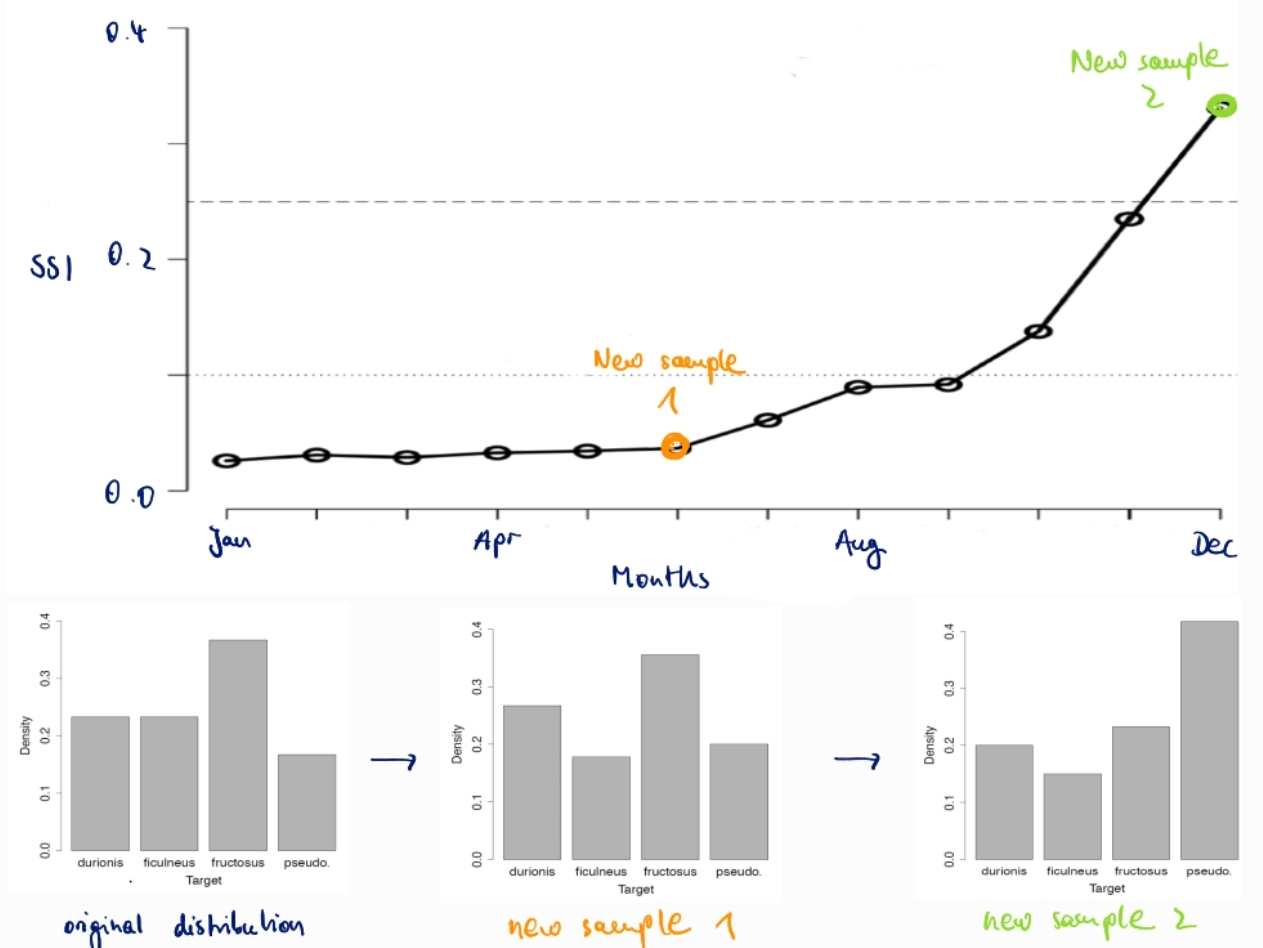
\includegraphics[width=\textwidth]{assets/sl/cd__ssi.jpg}
  \end{subfigure}

  \caption{System Stability Index: example}
  \label{fig:7_cd_ssi}
\end{figure}

